\chapter{CARACTERÍSTICAS TÉCNICAS}

Neste capítulo serão apresentadas características técnicas do Raspberry Pi, que podem ser lidas a seguir.

\section{Descrição técnica}

\begin{figure}[ht]
    \centering
    \scalebox{0.41}{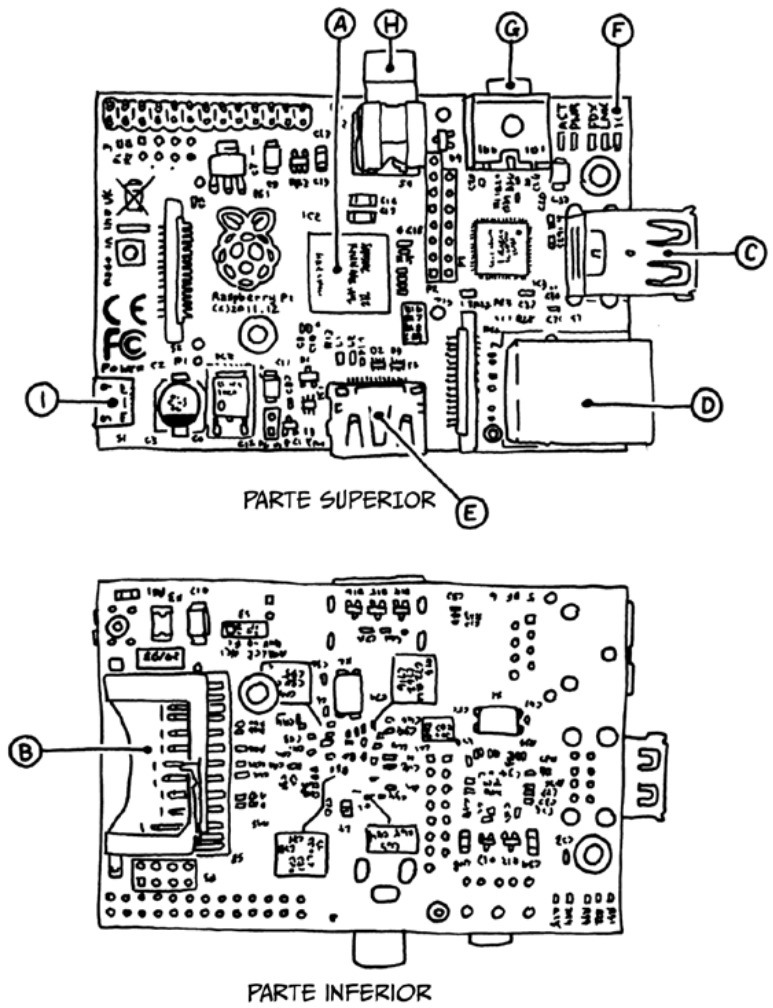
\includegraphics{figuras/superior_inferior}}
    \caption{Ilustração da placa Raspberry Pi}
\end{figure}

A figura 4.1 representação a placa do computador Raspberry Pi contendo indicações em diversos componentes, os quais serão melhor especificados a seguir.

\textbf{A. Processador.} No coração do Raspberry Pi está o mesmo processador que você encontraria no iPhone 3G e no Kindle 2, assim você pode pensar nas capacidades do Raspberry Pi como comparáveis a esses poderosos pequenos aparelhos. Este processador é sistema-em-um-chip de 700 MHz de 32 bits, construído sobre a arquitetura ARM11. Chips ARM apresentam-se em uma variedade de arquiteturas com diferentes núcleos configurados para fornecer diferentes capacidades com preços diferentes. O modelo B tem 512 MB de memória RAM e o modelo A tem 256 MB. (O primeiro lote do modelo B tinha apenas 256 MB de RAM.)
    
\textbf{B. Slot para cartão de memória SD (Secure Digital).} Você perceberá que não há disco rígido no Pi; tudo é armazenado em um cartão de memória SD. Uma razão pela qual você irá desejar, mais cedo ou mais tarde, algum tipo de gabinete (case) de proteção, é que as soldas no soquete SD poderão quebrar se o cartão for acidentalmente dobrado.

\textbf{C. Porta USB.} No modelo B há duas portas USB 2.0, mas apenas uma no modelo A. Algumas das primeiras placas do Raspberry Pi foram limitadas quanto à quantidade de corrente que elas poderiam fornecer. Alguns dispositivos USB podem chegar a 500mA. A placa original do Pi suportava 100mA ou quase, mas as revisões mais recentes alcançam até a especificação completa das portas USB 2.0. Provavelmente não é uma boa ideia recarregar seu celular com o Raspberry Pi. Você poderá usar um hub com alimentação externa se tiver um periférico que necessite de mais energia.

\textbf{D. Porta Ethernet.} O modelo B tem uma porta Ethernet padrão RJ45. O modelo A não tem, mas pode ser conectado a uma rede com fios por meio de um adaptador de rede Ethernet USB (a porta no modelo B é na verdade um adaptador Ethernet USB embutido). A conectividade Wi-Fi por meio de um adaptador USB externo (dongle) é outra opção.

\textbf{E. Conector HDMI.} A porta HDMI oferece saída de áudio e vídeo digital. Catorze resoluções de vídeo diferentes são suportadas, e o sinal HDMI, por meio de adaptadores externos, pode ser convertido para DVI (usado por muitos monitores), vídeo composto (sinal de vídeo analógico normalmente transmitido por um conector RCA amarelo), ou SCART (uma norma europeia para conexão de equipamentos audiovisuais).

\textbf{F. LEDs de status.} O Pi tem cinco LEDs indicadores de status que podem ser visualizados na Tabela 4.1 abaixo.

\newpage

\begin{table}[!htpb]
 \centering
    \begin{tabular}{|l|p{2cm}|l|} 
    \hline
        \textbf{Led} & \textbf{Cor} & \textbf{Descrição} \\
    \hline
        ACT & Verde & Acende quando o cartão SD é acessado \\
    \hline
        PWR & Vermelho & Conectado à alimentação de 3.3V \\
    \hline
        FDX & Verde & On (ligado) se o adptador de rede é full-duplex \\
    \hline
        LNK & Verde & Luz indicando atividade de rede \\
    \hline
        100 & Amarelo & On (ligado) se a conexão de rede for 100Mpbs \\
    \hline
    \end{tabular}
    \caption{LEDs com cindo indicações de status}
    \label{t_fixa}
\end{table}

\textbf{G. Saída de áudio analógico.} É um conector de áudio analógico padrão de 3,5 mm que é destinado a conduzir cargas de alta impedância (como alto-falantes amplificados). Fones de ouvido ou alto-falantes sem alimentação não terão som de qualidade. Parte desse problema tem a ver com o software controlador de áudio, o qual ainda está em desenvolvimento.

\textbf{H. Saída de vídeo composto.} É um conector-padrão tipo RCA que fornece sinais de vídeo composto NTSC ou PAL. Esses formatos de vídeo têm resolução extremamente baixa se comparada com HDMI. Se você tiver um monitor ou um televisor com entrada HDMI, use-o em vez de um televisor com entrada de vídeo composto.

\textbf{I. Entrada de energia.} Uma das primeiras coisas que você perceberá é que não há nenhum interruptor de alimentação no Raspberry Pi. Esse conector micro USB é usado para fornecer energia (essa não é uma porta USB adicional, é apenas para alimentação). A porta micro USB foi escolhida porque o conector é barato e fontes de alimentação USB são fáceis de encontrar.

\section{Periféricos adequados}

Após adquirir-se um pouco de conhecimento sobre os componentes da placa, faz-se necessário saber também sobre os periféricos adequados para utilizar com ela. A imagem abaixo mostra alguns dos quais iremos precisar para utilizar o Raspberry. É preciso tomar cuidado, pois existem peças que podem não funcionar corretamente quando instaladas na sua placa.

\begin{figure}[ht]
    \centering
    \scalebox{0.27}{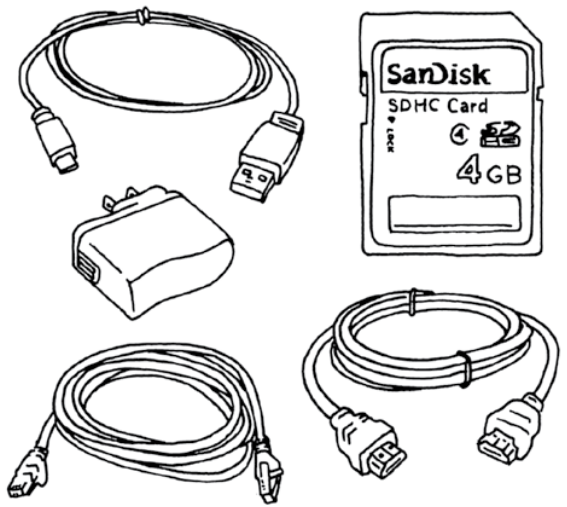
\includegraphics{figuras/perifericos_adequados}}
    \caption{Periféricos básicos: uma fonte de alimentação micro USB, cabos e cartão SD.}
\end{figure}

\textbf{Fonte de alimentação.} Este é o periférico mais importante para ser obtido. Você deve usar um adaptador micro USB que pode fornecer 5V e pelo menos 700mA de corrente (500mA para o modelo A). Um carregador de telefone celular não vai funcionar, mesmo se ele tiver o conector correto. Um carregador de telefone celular típico fornece apenas 400mA de corrente ou menos, mas verifique a classificação indicada na parte de trás. Um Raspberry Pi com fonte de alimentação inferior pode parecer funcionar, mas ficará estranho e poderá falhar (travar) de forma imprevisível. Um problema comum causado por insuficiência de corrente descrito pelos usuários do Raspberry Pi é que o teclado não funciona corretamente.

\textbf{Cartão SD.} Você vai precisar de pelo menos 4GB, e deve ser um cartão de Classe 4. Estes cartões são capazes de transferir pelo menos 4MB/seg. Algumas das placas anteriores do Raspberry Pi apresentaram problemas com cartões de Classe 6 ou superiores, os quais são capazes de velocidades mais rápidas, mas com menos estabilidade. Um cartão micro SD em um adaptador é perfeitamente utilizável também.

\textbf{Cabo HDMI.} Se você está se conectando a um monitor, precisará deste cabo ou um adaptador apropriado para um monitor DVI. Você também pode executar o Pi sem monitor, como descrito posteriormente neste capítulo. Cabos HDMI podem variar muito de preço. Se está instalando um cabo de 90 a 180 cm para o monitor, não há necessidade de gastar mais de US\$ 3 em um cabo HDMI. Se estiver instalando comprimentos maiores, você definitivamente deve pesquisar cabos de maior qualidade e evitar os genéricos mais baratos.

\textbf{Cabo Ethernet.} Sua casa pode não ter mais tantos conectores Ethernet com fio como tinha há cinco anos. Visto que atualmente praticamente tudo é sem fio (wireless), você pode encontrar um pouco de dificuldade com a porta com fio (cabeada).

\newpage

\section{Outras características}

Na tabela a seguir são apresentadas mais algumas características do Raspberry Pi.

\begin{table}[!htpb]
 \centering
    \begin{tabular}{|p{4cm}|c|c|} 
    \hline
        \textbf{Funcionalidade} & \textbf{Suportado pelo Raspberry Pi} & \textbf{Não Suportado pelo Raspberry Pi} \\
    \hline
        Imprime em impressora local? & X & \\
    \hline
        Imprime em rede? & X & \\
    \hline
        Serve arquivos em rede? & X & \\
    \hline
        Executa java? & X & \\
    \hline
        Executa ruby? & X & \\
    \hline
        Executa python? & X & \\
    \hline
        Serve impressora? & X & \\
    \hline
        Edita textos, planilhas, apresentações? & X & \\
    \hline
    \end{tabular}
    \caption{Outras características do Raspberry Pi}
    \label{t_fixa}
\end{table}
